\documentclass[hidelinks, a4paper,11pt,twoside]{report} % Please disable the twocolumn later
\usepackage{font/fin} %<- Contains all formatting stuff! % Ensure you are using rpb_fin.sty
\usepackage[switch]{lineno} %\linenumbers % Place line on the side

\setcounter{tocdepth}{3} \brokenpenalty=10000 \tolerance=1 \emergencystretch=\maxdimen \hyphenpenalty=10000 \hbadness=10000

% Start to enable during final version
\renewcommand{\cfttabfont}{Table } % Do not change, To allow in TOC for text appear with Table 1.2 xxx
\renewcommand{\cftfigfont}{Figure } % Do not change, To allow in TOC for text appear with Figure 1.2 xxx
% End to enable during final version

% Start Package for table
\usepackage{makecell}
\newcolumntype{P}[1]{>{\centering\arraybackslash}p{#1}}
\newcolumntype{M}[1]{>{\centering\arraybackslash}m{#1}}

% From https://tex.stackexchange.com/questions/241892/two-figures-side-by-side-caption
\usepackage{floatrow}

% From https://tex.stackexchange.com/questions/22751/how-to-force-table-caption-on-top
% Forcing table caption on top
\floatsetup[table]{capposition=top}

% See: https://tex.stackexchange.com/questions/340433/formatting-table-with-siunitx-problem-with-special-format
\usepackage{booktabs,siunitx} 
\sisetup{table-format=2.1}
% End Package for table

% Start graphic package
\usepackage{graphicx}
\newcommand{\plus}{\raisebox{.4\height}{\scalebox{.6}{+}}}
\graphicspath{ {./images/} }

\usepackage[caption=false]{subfig}
% End graphic package

% Start Math package
\usepackage[cmex10]{amsmath} 
\DeclareMathOperator*{\argmax}{argmax}
\usepackage{scalerel,amssymb}
% End Math package

\def\msquare{\mathord{\scalerel*{\Box}{gX}}}
\def\msbigtriangledown{\mathord{\scalerel*{\bigtriangledown}{gX}}}
\def\mcirc{\mathord{\scalerel*{\bigcirc}{gX}}}

% APA citation settings
\usepackage{csquotes} % Recommended for biblatex with APA style
\usepackage[style=apa, backend=biber, natbib]{biblatex} 
\DeclareLanguageMapping{english}{american-apa}
\addbibresource{BibThesis.bib} % Link to your .bib file

\usepackage{url}
\usepackage{hyperref} % Ensure hyperref is loaded

% Shortcut
\usepackage{xspace} % Solve the spacing issue

\usepackage{setspace} % Modify the double/single spacing

\usepackage[open,openlevel=2]{bookmark}

\hyphenation{appli-cability}

\begin{document}

\pagestyle{plain}\cleardoublepage %To Add empty page and start on odd number (SOFTBOUND)%%

\include{chap0_FrontPage.tex}
\raggedbottom 

\title{INOVATIVE: TO CREATE NEW MODULE FOR EFFECTIVENESS IN ADMINISTRATIVE STAFF WORKFLOW BY USING FULLY SISTEMIZE APPLICATION}

\TitleMalay{INOVATIF: MEWUJUDKAN MODUL BARU DALAM MENINGKATKAN KEBERKESANAN PROSES KERJA KAKITANGAN PENTADBIRAN DENGAN MENGGUNAKAN SEPENUHNYA APLIKASI BERSISTEMATIK}



\abstract{The acquisition of new vocabulary in a second language requires a series of repeated exposures. With emerging digital platforms and games such exposure can easily be provided. Due to the prevalence and ease of access of mobile technology, learners have demonstrated a high degree of dependence on digital tools such as smartphones for learning as compared to traditional approaches. This study is aimed at exploring whether a game-based thesaurus app could be used to improve the level of English language vocabulary among students in a public university in Malaysia. The findings reveal that students have less experience on using thesaurus apps compared to games or other language learning apps. Students prefer the use of mobile learning over traditional approach, prefer online platforms rather than mobile apps, and acquire or build up their vocabulary through watching movies and listening to music. Even though most students have adequate experience using mobile apps and games, they rarely use those platforms for learning purposes. This suggests that it is crucial to incorporate game elements into learning platforms particularly in learning English vocabulary to generate motivation and engagement to learners. Lecturers should therefore focus more on the explicit use of mobile digital technology in their teaching and learning classrooms. }



\abstractMalay{Pemerolehan perbendaharaan kata baharu dalam bahasa kedua memerlukan satu siri pendedahan berulang kali. Melalui platform digital dan permainan yang baru, pendedahan tersebut boleh disediakan dengan mudah. Oleh kerana kelaziman dan akses teknologi mudah alih adalah senang, pelajar telah menunjukkan tahap kebergantungan yang tinggi terhadap alat digital untuk belajar, seperti melalui telefon pintar berbanding dengan pendekatan tradisional. Kajian ini bertujuan untuk meneroka sama ada aplikasi tesaurus berasaskan gamificasi boleh digunakan untuk memperbaiki tahap penguasaan perbendaharaan kata dalam Bahasa Inggeris dalam kalangan pelajar universiti awam di Malaysia. Hasil kajian menunjukkan bahawa pelajar mempunyai pengalaman yang kurang dalam menggunakan aplikasi tesaurus berbanding pembelajaran bahasa berasaskan permainan atau aplikasi lain. Pelajar lebih suka menggunakan pembelajaran mudah alih berbanding pendekatan tradisional, lebih suka platform dalam talian dan bukannya aplikasi mudah alih, dan memperoleh atau membina perbendaharaan kata mereka melalui menonton filem dan mendengar muzik. Meskipun fakta menyatakan bahawa kebanyakan pelajar mempunyai pengalaman yang mencukupi dalam penggunaan aplikasi mudah alih dan permainan, namun mereka jarang menggunakan platform tersebut untuk tujuan pembelajaran. Ini menunjukkan bahawa adalah penting untuk menggabungkan elemen permainan ke dalam platform pembelajaran khususnya dalam pembelajaran perbendaharaan kata Bahasa Inggeris sebagai satu cara untuk menjana motivasi dan penglibatan pelajar. Oleh yang demikian, pensyarah perlu memberi tumpuan lebih kepada penggunaan yang jelas terhadap teknologi digital mudah alih dalam pengajaran dan pembelajaran di bilik darjah. }


\author{RODNEY PETRUS BALANDONG}
% \programfacul{INDUSTRIAL PHYSICS}
% \faculty{FACULTY OF SCIENCE AND NATURAL RESOURCES}


\degree{ BACHELOR OF SCIENCE WITH HONORS} % or \degree{Master of Science} 
\mainsupervisor{AP. Dr. Zoro}



\matricno{2023456}


\copyrightyear{\number\the\year} % or \copyrightyear{20xx}


\declarationLLM{I acknowledge that during the preparation of this thesis, I have utilized Large Language Models (LLMs) as a supplementary tool to assist in various aspects of my research and writing process. Specifically, I have used LLMs for paraphrasing and refining my writing to improve clarity, coherence, and readability while ensuring the original meaning remains intact. Additionally, I have leveraged LLMs to generate general ideas and structure my thoughts more effectively, using them as a brainstorming aid rather than as a replacement for original critical thinking. LLMs have also been helpful in summarizing complex topics, identifying key points from lengthy articles, and suggesting alternative ways to present information. Furthermore, I have used LLMs to check grammar and syntax, ensuring that my writing adheres to academic standards. In some instances, LLMs provided guidance on citation formats and referencing best practices, although all sources have been manually verified to maintain academic integrity. Importantly, I have critically evaluated all AI-generated content and ensured that it aligns with my own understanding and research findings.}


\penghargaan{It is good to tha}

%%%%% IMPORTANT. DO NOT PLACE WHAT HAVE BEEN DECLARED ABOVE, AFTER THIS CELL
\beforepreface %dont change this

\afterpreface  %don't change this
\chapter{INTRODUCTION}



The introduction chapter of a thesis sets the stage for the entire research, providing the reader with essential background information, the context of the study, and a clear outline of the research objectives and significance. Each section within the introduction builds upon the previous one, gradually guiding the reader toward understanding the research problem and the purpose of the study. This section can be divided in multiple subsection to organize the information logically.

\section{Background}

In this section \parencite{Lal_2005as, Vassalli2009}, you aim to provide the reader with the foundational knowledge necessary to understand the broader context of your research. This includes explaining key concepts, relevant terminology  \parencite{Amso_2015}.


\begin{figure}
	\centering
	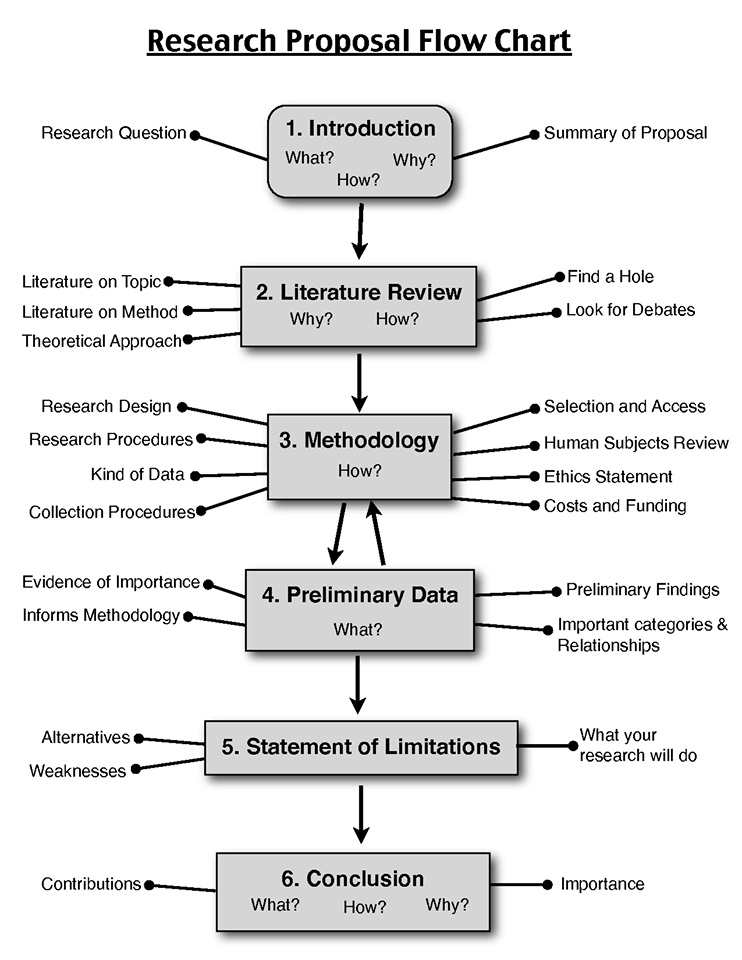
\includegraphics[width=15cm]{Writing research research proposal.png}
	\caption[Research Proposal Flow Chart]
	{The image is a flow chart titled "Research Proposal Flow Chart," designed to guide the development of a research proposal through six key stages: Introduction, Literature Review, Methodology, Preliminary Data, Statement of Limitations, and Conclusion. Each stage addresses specific questions like "What?", "Why?", and "How?", ensuring a comprehensive and structured approach. The chart outlines the progression from defining the research question and reviewing relevant literature, to detailing the methodology, presenting preliminary data, discussing limitations, and concluding with the significance of the research. This visual tool is essential for researchers in planning and articulating their study in a coherent and logical manner.. Figure adapted from \cite{Dorsett2010}.}
	\label{fig:ExxonSpreading}
\end{figure}
%

\begin{table}[h]
    \centering
    \begin{tabular}{|c|c|c|}
        \hline
        \textbf{Column 1} & \textbf{Column 2} & \textbf{Column 3} \\
        \hline
        Data 1 & Data 2 & Data 3 \\
        Data 4 & Data 5 & Data 6 \\
        Data 7 & Data 8 & Data 9 \\
        \hline
    \end{tabular}
    \caption{Simple Table Example}
    \label{tab:simple_table}
\end{table}
\subsection{Concept and Terminology Explanation}

In this subsection, you should broadly explain the key concepts and terminology that are central to your research. This will help ensure that readers who are not familiar with the topic can follow along.




\section{ Importance and Relevance} 
\label{SplitScheduleExplain}

In this subsection, explain why the topic is important and relevant. Include statistics, the impact of the topic on society, and any related government policies or initiatives. This helps to justify why your research is necessary and valuable.




\section{Motivation}

The motivation section of a thesis is crucial as it articulates the rationale behind the research, highlighting its importance and relevance. This section will help connects the background information with the research objectives by explaining why the study is necessary and what gaps it aims to fill. 

This section (and its subsection) builds a compelling case for the research by discussing the potential benefits and impact of the findings, thereby justifying the effort and resources invested in the study. The motivation section ensures that the reader understands the significance of the problem being addressed and the value that the proposed solutions can bring to the field.

You can give a brief overview or compact explaination from the literature review, what is there, but what is still missing. or the justification of why you insist of using some technique


\subsection{Some subsection to decompose your explaination}




\section{Problem Formulation}


\subsection{Research Gap}

The identified gap based on your literature review


\subsection{Problem Statement}

Based on the research gap, the following problems have been identified:

\begin{enumerate}
    \item \textbf{Definition of the Problem:} The problem statement clearly defines the issue that the research aims to address. It should describe the gap in knowledge, real-world challenges, or theoretical inconsistencies that necessitate investigation.

    \item \textbf{Relation to Hypotheses:} The problem statement serves as the foundation for formulating hypotheses. It outlines the research issue, while the hypotheses provide testable predictions based on this problem.

    \item \textbf{Best Practices for Writing a Problem Statement:}
    \begin{itemize}
        \item \textbf{Be clear and concise:} The problem statement should be straightforward, avoiding unnecessary jargon while effectively communicating the research issue.
        \item \textbf{Explain the research gap:} Clearly identify what is missing in existing research and why addressing this gap is important.
        \item \textbf{Define the scope:} Specify the boundaries of the problem, ensuring that it is neither too broad nor too narrow.
        \item \textbf{Highlight significance:} Explain why solving this problem is important, including its potential impact on the field, industry, or society.
        \item \textbf{Use evidence to support the problem:} Reference previous studies, statistics, or real-world examples to justify why the problem exists and why it requires investigation.
        \item \textbf{Ensure alignment with research objectives:} The problem statement should align with the study’s aims, ensuring consistency throughout the research process.
    \end{itemize}
\end{enumerate}


\section{Hypotheses of Study}
Based on the depicted problem statement, the following have been hypothesised:

\begin{enumerate}
    \item \textbf{Hypotheses:} A hypothesis is a testable statement or assumption that predicts the relationship between variables in a study. It serves as the foundation for research by providing a direction for investigation.

    \item \textbf{Relation to Problem Statement:} The problem statement defines the research issue and its significance, while hypotheses emerge from it as specific, testable propositions. The hypotheses offer potential explanations or solutions to the problem and guide data collection and analysis.

    \item \textbf{Best Practices for Writing Hypotheses:}
    \begin{itemize}
        \item \textbf{Be clear and specific:} A hypothesis should be precise and unambiguous, defining the variables and their expected relationship.
        \item \textbf{Ensure testability:} A good hypothesis should be measurable and testable using empirical methods.
        \item \textbf{Base it on existing knowledge:} Formulate hypotheses based on prior research, theories, or observations.
        \item \textbf{Use an "If-Then" structure (if applicable):} For causal relationships, use an "If X, then Y" format to establish a clear cause-and-effect relationship.
        \item \textbf{Make it falsifiable:} A hypothesis should be structured in a way that allows it to be proven false if the evidence contradicts it.
        \item \textbf{Keep it simple and focused:} Avoid overly complex hypotheses by keeping them concise and to the point.
    \end{itemize}
\end{enumerate}



\section{Research Question}

\begin{description}
    \item[RQ3] - Is there any significant correlation between social presence and course satisfaction among third-year Malaysian undergraduates undertaking a BL course in UMS?
    \item[RQ4] Is there any significant correlation between cognitive presence and course satisfaction among third-year Malaysian undergraduates undertaking a BL course in UMS?
    \item[RQ5] Which factor of teaching, social, and cognitive presence is dominant in determining course satisfaction among third-year Malaysian undergraduates undertaking a BL course in UMS?
\end{description}

\section{Study Objectives}



Based on the hypotheses, the following research objectives have been formulated:

\begin{enumerate}    
    \item  You may refer to online sources about SMART objectives, which define a goal that is specific, measurable, achievable, relevant, and time-bound.


       


    
\end{enumerate}



\section{Scope Of Work}

The scope of work for this thesis are:

\begin{enumerate}    


	
\end{enumerate}

\section{Organisation Of Thesis}
\label{ThesisOrganisation}


\noindent The organisation of this thesis is elaborated in the following:

Chapter 1 serves as an introduction, providing an overview of the study and emphasizing the importance of ... . You may eloborate more

Chapter 2 discusses relevant background information on.. . You may eloborate more

Chapter 3 details the development of the proposed method. You may eloborate more

Chapter 4 presents the experimental analysis and validation of the proposed . You may eloborate more

Chapter 5 summarizes key findings from each chapter, highlights the research contributions of this thesis in advancing.. You may eloborate more


The Chapter Appendix includes detailed explanations of the s. 



\clearpage

\begin{singlespace}
	\setstretch{1} % Adjust this value for bibliography readability
	\smallskip
	\printbibliography[heading=bibintoc, title=REFERENCES] % Print bibliography in APA style
\end{singlespace}

\end{document}
